\documentclass[12]{article}
\usepackage{graphicx}
\usepackage{wrapfig}

\begin{document}

The product is also called \textbf {\underline{dot product}} or \textbf { \underline {inner product} }, and also denoted by $ A | B $, $ ( A , B )$, $< A , B >$ or $ \ll A,B \gg $.

The scalar product $ \mathrm{A} \cdot \mathrm{B} $ certainly vanishes when $\mathrm{A} = 0 $ or $\mathrm{B} = 0 $. For nonzero vectors, the product is positive, zero or negative according as $\theta$ is an acute, right or obtuse angle. \\


\underline{Geometric Interpretations:} \\

\begin{wrapfigure}{R}{0.3\textwidth}
	\centering
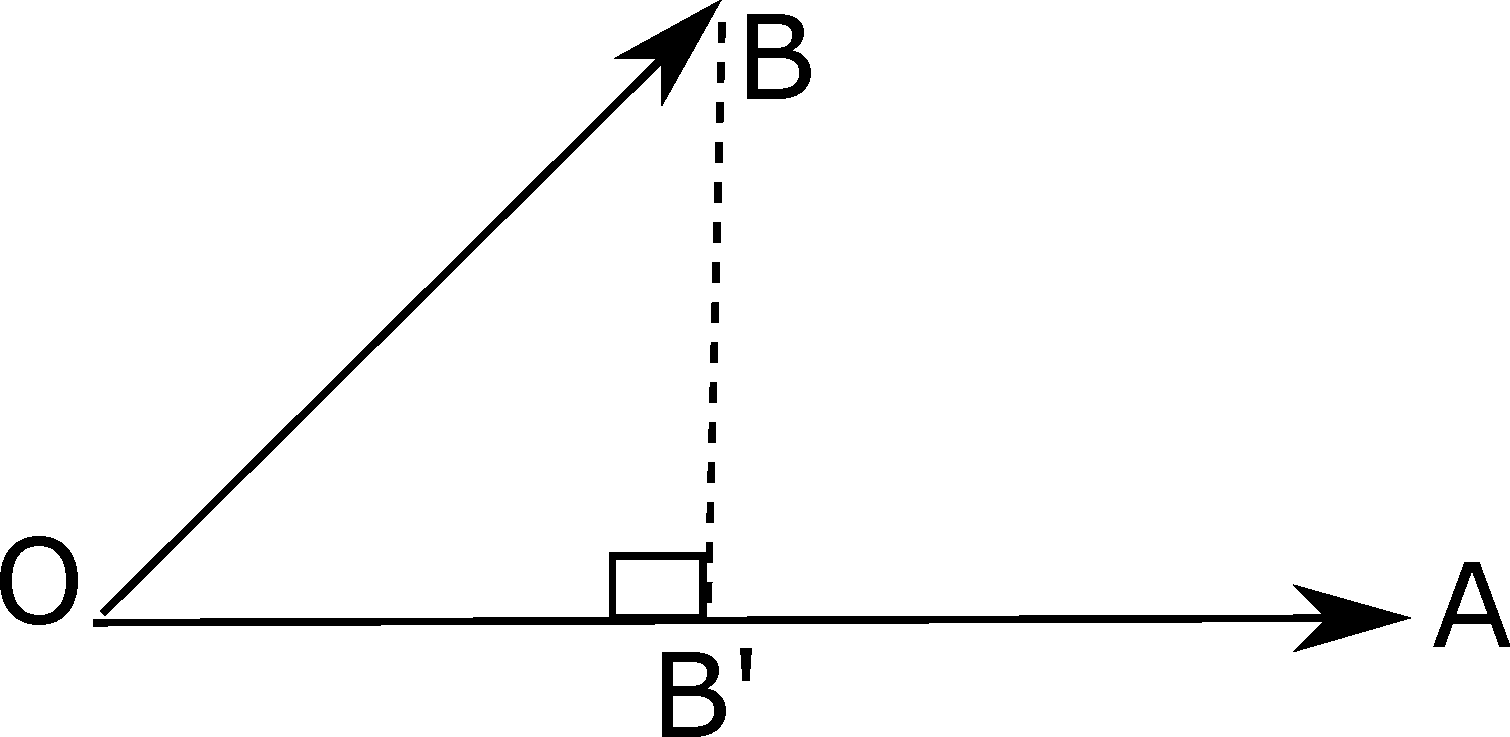
\includegraphics[width=0.25\textwidth]{drawing1}
\end{wrapfigure}
 
1.  If $ \mathrm{ \vec{{OB'}}} $ is the projection of $ \mathrm{ \vec{OB} } $ on $ \mathrm{ \vec{OA} }$, then\\

$ \mathrm{ \vec{OA} \cdot \vec{OB} } = \mathrm{ \vec{OA} \cdot \vec{OB'} } $\\
\begin{wrapfigure}{R}{0.2\textwidth}
	\centering
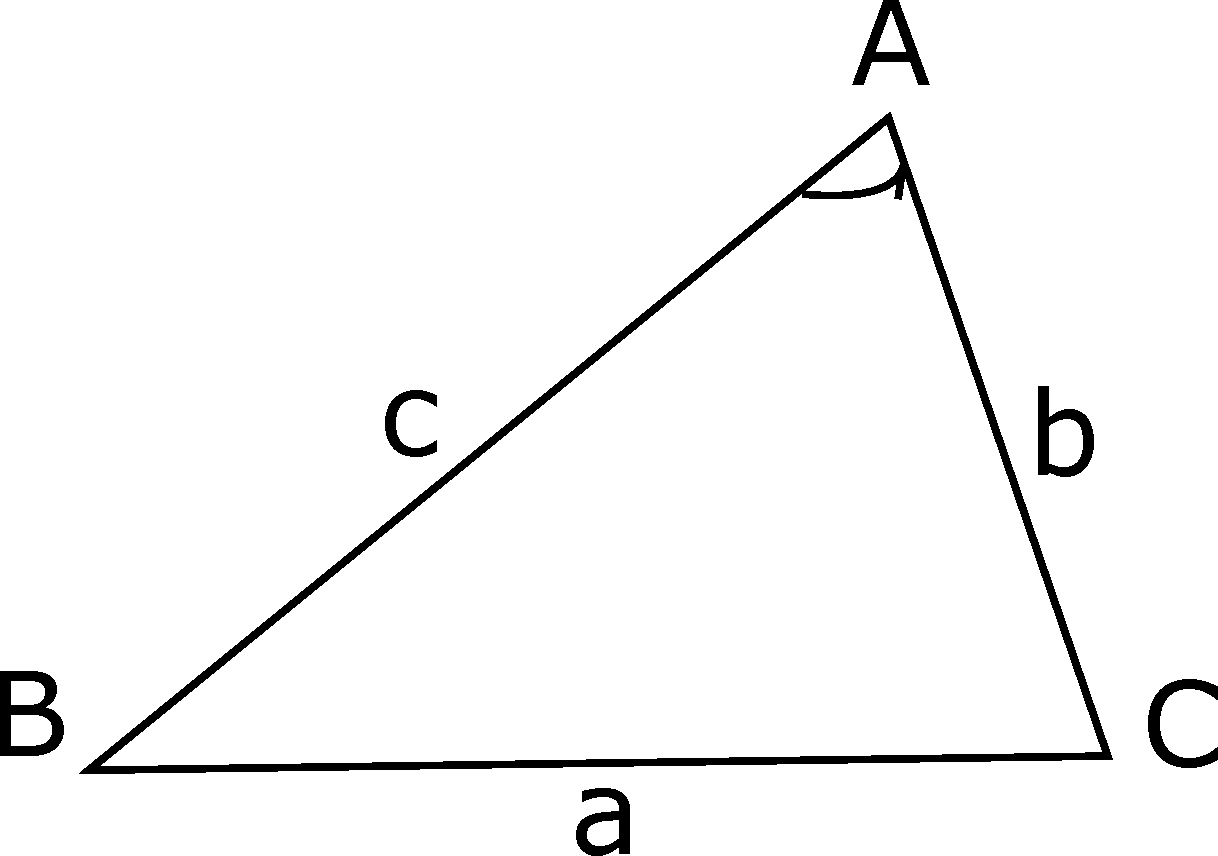
\includegraphics[width=0.25\textwidth]{drawing2}
\end{wrapfigure}\\


2.  The cosine law $ a^2 = b^2 + c^2 - 2bc \cos \alpha $ for a triangle $\ mathrm{ABC} $ can be expressed in the form\\

$ \mathrm{ |BC|^2 = |AB|^2 + |AC|^2 - 2 \vec{AB} \cdot \vec{AC} } $ \\


3.  Two nonzero vectors are perpendicular (orthogonal) if and only if their dot product is zero: \\
$$ \mathrm{ A \perp B \iff \theta = 
									\frac
									{\Pi}{2}
						\iff A \cdot B = 0 }$$

4.  The dot product of two vectors with known lengths (of variable directions) is maximum or minimum when they are parallel in the same or opposite senses.\\

\underline{Physical Interpretation:}
\begin{wrapfigure}{R}{0.3\textwidth}
	\centering
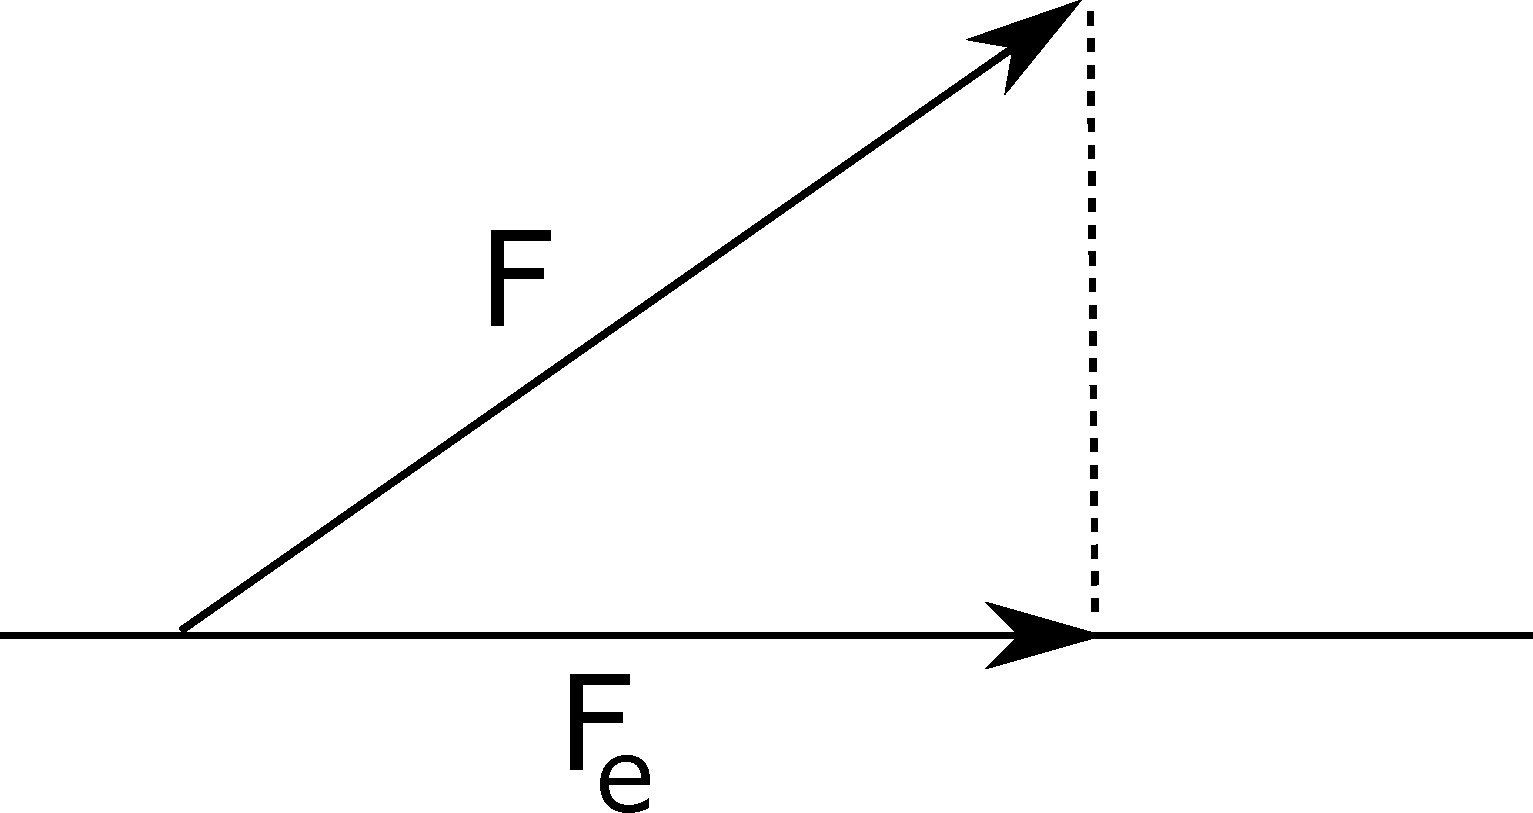
\includegraphics[width=0.3\textwidth]{drawing3}
\end{wrapfigure}\\


If a particle is moving on a line in the direction of a vector $ \mathrm{ \vec{R} }$, under a force $ \mathrm{ \vec{F} } $ then the effective force $\mathrm{ \vec{F_e} } $ is the projection vector of $ \mathrm{ \vec{F} } $ on $\mathrm{ \vec{R} } $ in the direction of motion: \ \ $ \mathrm{ \vec {F} \cdot \vec{R} =\vec{F_e} \cdot \vec{R} } $.

\end{document}